\documentclass[12pt]{article}

\input{0a - preambule}
\title{\textit{Pourquoi} la surface d'un disque est $\pi r^2$ ?}

\begin{document}

\maketitle

Un disque de rayon $r$ a pour périmètre $2\pi \times r$. \\
Découpons ce disque en quartiers:

\begin{center}
    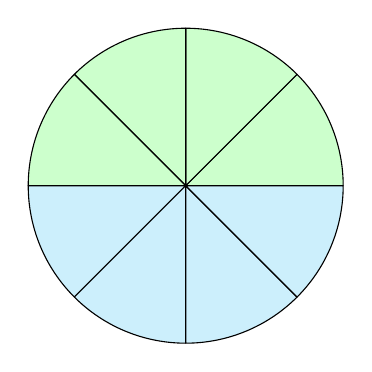
\begin{tikzpicture}[line join=round, line cap=round]
        \foreach \k in {0, ..., 7} {
            \ifnum\k>3 \def\couleur{cyan!20} \else \def\couleur{green!20} \fi
        
            \path[draw=black, fill=\couleur]
                (45*\k:2) arc[start angle=45*\k, end angle=45*(\k+1), radius=2]
                -- (45*\k:0)
                -- cycle;
        }
    \end{tikzpicture}
\end{center}

Et assemblons les verticalement: la somme des longueurs des arcs de cercle à gauche ou à droite vaut un demi-périmètre, soit $\pi r$. La longueur des segments constituant chaque quartier vaut $r$, le rayon du cercle.

\tikzset {
    pics/camemberts/.style args={#1} {
        code={
            \def\R{2.0} % rayon
            \def\n{#1} % nombre de secteurs empilés
            \def\phi{180/\n} % demi-angle du secteur (en degrés) -> ouverture = 2*phi
        
            \pgfmathsetmacro{\dy}{\R*sin(\phi)}
            \pgfmathsetmacro{\dx}{(\R/2)*cos(\phi)}
          
            \foreach \k in {0,...,\numexpr\n-1\relax} {
                \ifodd\k
                    \def\couleur{green!20}
                    \def\signe{1}
                \else
                    \def\couleur{cyan!20}
                    \def\signe{-1}
                \fi
        
                \coordinate (V) at (-\signe*\dx, \k*\dy); % sommet du secteur
        
                % secteur: sommet -> rayon bas -> arc extérieur -> retour sommet
                \path[draw=black, fill=\couleur]
                    (V) -- ++(-\phi:\R*\signe)
                    arc (-\phi:+\phi:\R*\signe)
                    -- cycle;
            }
            
            \coordinate (B) at (-\dx-\R/5, -\dy);
            \coordinate (H) at (-\dx-\R/5, \n*\dy-\dy);
            \draw[<->] (H) -- (B)
                node[midway, left] {$\pi \times r$};

            \draw[<->] (-\dx, -\dy-\R/5) -- (\R + -\dx, -\R/5)
                node[midway, below] {$r$};
                
        }
    }
}

\begin{center}
    \begin{tikzpicture}
        \pic {camemberts={8}};
    \end{tikzpicture}
\end{center}

Découpons les cercles en 32 et 128 parts: plus le nombre de parts augmente, plus l'assemblage s'approche d'un rectangle de hauteur $\pi r$ et de largeur $r$, donc plus la surface s'approche de $\pi r^2$

\begin{center}
    \begin{tikzpicture}
        \pic at ($(0, 0) + (3/6*\linewidth, 0)$) {camemberts={32}};
        \pic at ($(0, 0) + (5/6*\linewidth, 0)$) {camemberts={128}};
    \end{tikzpicture}
\end{center}

Autrement dit, lorsque que le nombre de parts tend vers l'infini ($+\infty$), la forme résultant tend vers un rectangle de hauteur $\pi \times r$ et de largeur $r$, donc de surface $\pi \times r^2$.

\end{document}